\documentclass[dvips,plainheader,pnumromarab]{abnt}
\usepackage[brazil]{babel}
% \usepackage[latin1]{inputenc}
\usepackage[utf8]{inputenc}
\usepackage[pdftex]{graphicx}
% \usepackage[pdftex]{hyperref}
\usepackage{abnt-alf}
\usepackage{latexsym}
\usepackage{psfrag}
\usepackage{setspace}
% \usepackage[center]{caption2}
\usepackage{epigraph}

% Gloss�rio n�o utilizado
% \usepackage{makeglo}
% \renewcommand{\glossaryname}{Gloss�rio}
% \makeglossary

\begin{document}

\DeclareGraphicsRule{.eps.gz}{eps}{.eps.bb}{`gunzip -c #1}

% \begin{figure}[htp]
	\centering
	\includegraphics[scale=1.5]{Figuras/capa}
% 	\caption{Tentativas de Fraudes Reportadas - 2012}
% 	\label{fig:estatisticas-fraudes-reportadas}
\end{figure}
\titulo{Fragmentação de Arquivos em File Carving em Sistemas de Arquivos NTFS}
\autor{Márcio Fernandes Justino}
\orientador[Orientadora:\\]{Ivete Irene dos Santos}
\comentario{Projeto de pesquisa apresentado como requisito parcial para a aprovação na disciplina Metodologia do Trabalho Científico do Curso de Computação Forense da Universidade Presbiteriana Mackenzie.}
\instituicao{Universidade Presbiteriana Mackenzie \par
Instituto de Computação \par
Pós Graduação em Computação Forense}
\local{São Paulo -- SP}
\data{Maio / 2013}
\capa
\folhaderosto
\ 

\vfill

\begin{flushright}
\hfill \textit{Dedico a meus pais, cujo exemplo\\ de honestidade e trabalho tem marcado\\ minha vida, à minha esposa que me apoiou\\nesta caminhada e à minha filha que\\ acompanhou todo este trabalho\\ ainda no ventre da mãe.}
\end{flushright}

\vspace*{1cm}

\clearpage

\begin{resumo}

%*****************************************************************************************************
% Apresenta��o concisa dos pontos relevantes, dando uma vis�o r�pida e clara do conte�do do trabalho.
%*****************************************************************************************************
A fragmenta��o de arquivos tem sido o calcanhar de Aquiles dos processos investigativos e per�cias forenses envolvendo a recupera��o de arquivos e,
principalmente, de arquivos n�o mais alocados, removidos ou corrompidos. A abordagem do tema tem caminhado para um avan�o nos processos de localiza��o
dos fragmentos de arquivos e seus diferentes tipos de t�cnicas, possibilitando que as ferramentas evoluam cada vez mais no processo de
identifica��o e localiza��o de arquivos fragmentados, auxiliando assim na investiga��o mais robusta e eficiente de evid�ncias digitais.

\textbf{Palavras-chave:} Fragmenta��o, investiga��o, arquivos, t�cnicas, evid�ncias.

\end{resumo}

\tableofcontents

\chapter{Introdu��o}
Juntamente com o avan�o da tecnologia computacional e da internet, veio o aumento do n�mero de pessoas conectadas trocando informa��es, seja em n�vel pessoal ou organizacional. Segundo o Centro de Estudos sobre as Tecnologias da Informa��o e da Comunica��o (cetic.br), o n�mero de usu�rios dom�sticos e no trabalho tem aumentado juntamente com o tempo em que os mesmos permanecem conectados � internet. A figura \ref{fig:fig01} mostra a evolu��o desses n�meros at� o presente momento.

\begin{figure}[htp]
  \centering
  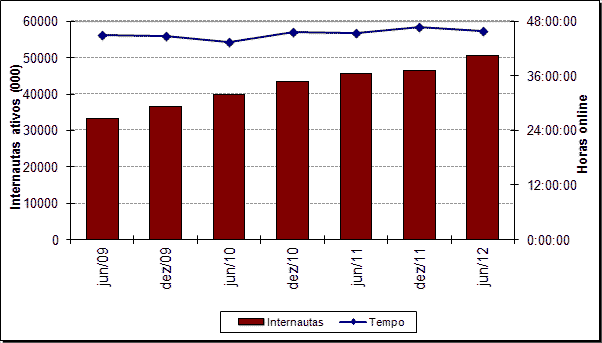
\includegraphics[scale=0.6]{figuras/fig01.png}
  \caption{Internautas ativos em resid�ncias e no trabalho e horas navegadas - 2012 \cite{CeticBR2012}}
  \label{fig:fig01}
\end{figure}

Nesse meio, existem usu�rios que promovem o cibercrime\footnote{crimes cibern�ticos tendo sistemas informatizados como meio de a��o \cite{CyberCitizen2012}.} ou atividades ilegais na rede\footnote{o termo rede ser� usado ao longo deste texto podendo representar a internet como um todo ou a liga��o de mais de computadores entre si.}. As informa��es computacionais s�o armazenadas em discos r�gidos\footnote{unidade f�sica de armazenamento de dados em um computador} usando apropriados sistemas de arquivos que s�o suportados pelo sistema operacional instalado no computador. Existem diversos sistemas de arquivos para armazenamento de arquivos no mercado, e um dos mais comuns atualmente � o NTFS \cite{Meshram2012}.

\begin{citacao}
``O sistema de arquivos NTFS, assim como outros sistemas de arquivos, n�o foi criado com a computa��o forense em mente mas sim com a quantidade de informa��es no computador que pode ser usada em uma investiga��o'' \cite[p.~32]{Svensson2005}
\end{citacao}

Muitos criminosos se utilizam do artif�cio de excluir ou remover rastros de seus atos criminosos apagando os arquivos criados, manipulados ou alterados, acreditando que com isso seu crime seria perfeito, sem rastros da comprova��o de seus atos. A t�cnica de file carving possibilita a an�lise de tais arquivos, provendo um avan�o investigativo  com a possiblidade de extrair provas de arquivos n�o mais alocados, por�m que ainda estejam presentes fisicamente nos discos.

Segundo Caloyannides (2004, p. 26), a opera��o de remo��o de um arquivo n�o faz absolutamente nada. Esta meramente altera um simples caractere na tabela de aloca��o do arquivo em quest�o indicando ao computador que o espa�o desse arquivo foi tomado permitindo que os dados do arquivo possam ser sobrescritos no futuro, se necess�rio. Seguindo racioc�nio semelhante, a opera��o de formata��o n�o remove os dados sens�veis dos arquivos. A formata��o faz com que os ponteiros da tabela de aloca��o que indicam onde os arquivos est�o sejam liberados, perdendo assim sua localiza��o pelo sistema de arquivos, mas mantendo os dados intactos em seu sistema. De acordo com Caloyannides (2004, p. 33), os arquivos s�o alocados no disco em unidades m�nimas chamadas clusters\footnote{Unidade m�nima que pode ser acessada pelo sistema de arquivos, constitu�do de setores e de tamanho vari�vel dependendo do sistema de arquivos e da op��o de formata��o.}. Se o sistema de arquivos n�o necessita de todo o cluster 
para armazenar as informa��es do arquivo, este ir� marcar o final do arquivo na por��o final de seus dados dentro do cluster, deixando uma por��o do cluster com dados considerados lixo, n�o sobrescritos pelo sistema. Essa situa��o gera o que � chamado de slack space\footnote{Espa�o n�o alocado em um cluster que pode conter informa��es de outros arquivos que n�o foram sobrescritas.}. Por fim, o processo de formata��o e remo��o de um arquivo, juntamente com as �reas de slack space do disco, provoca o surgimento de �reas n�o alocadas, o que caracteriza o processo de file carving.

\section{Justificativa}
Segundo Memon (2011, p. S2), um dos primeiros desafios em file carving pode ser encontrado na tentativa de se recuperar arquivos fragmentados. O processo de file carving � de suma import�ncia para a investiga��o forense computacional e envolve a identifica��o de arquivos perdidos, corrompidos ou removidos do equipamento investigado. A dispers�o desses arquivos n�o mais indexados pela tabela de aloca��o de arquivos do sistema de arquivos NTFS torna o processo de identifica��o dos arquivos um desafio para a investiga��o e identifica��o de il�citos.

\begin{citacao}
``Durante uma investiga��o forense digital, muitas pe�as diferentes de dados s�o preservadas para investiga��o, das quais imagens de discos r�gidos (HD's) s�o as mais comuns. Essas imagens cont�m os dados alocados para arquivos, bem como os dados n�o alocados. Os dados n�o alocados ainda podem conter informa��es relevantes para uma investiga��o, sob a forma de (partes de) intencionalmente exclu�dos ou arquivos tempor�rios removidos automaticamente. Infelizmente, esses dados nem sempre s�o facilmente acess�veis: uma sequ�ncia de caracteres da pesquisa sobre os dados brutos pode recuperar (partes de) documentos de texto interessantes, mas ele n�o vai ajudar para obter a informa��o presente em, por exemplo, imagens ou arquivos compactados. Al�m disso, as sequ�ncias de caracteres exatas para procurar n�o podem ser conhecidas antecipadamente. Para obter esta informa��o, os arquivos apagados precisam ser recuperados'' \cite[p.~1]{Kloet2007}.
\end{citacao}

\section{File Carving}
A t�cnica de file carving � frequentemente utilizada durante investiga��es digitais. Conforme Memon (2011, p. S2), essa � uma t�cnica em que arquivos de dados s�o extra�dos de um dispositivo digital sem o aux�lio de tabelas de arquivo ou outros meta-dados do disco. 

\begin{citacao}
``Na pratica forense, o processo de file carving pode recuperar arquivos que foram removidos e que tiveram sua entrada de diret�rio realocada para outros arquivos, desde que seus setores de dados n�o tenham sido sobrescritos ainda'' \cite{Garfinkel2007}.
\end{citacao}

\section{Fragmenta��o de Arquivos}
Conforme Menom (2011, p. S2), um dos primeiros desafios do processo de investiga��o utilizando file carving � justamente a tentativa de recuperar os fragmentos de arquivos n�o alocados. A fragmenta��o de arquivos � um desafio para o processo de file carving e � de suma import�ncia para a recupera��o de arquivos perdidos em processos de investiga��o digital. Tendo em vista o presente desafio, tem-se a necessidade de se determinar qual a melhor t�cnica para identifica��o de fragmentos de arquivos no processo de file carving.

\section{Hip�tese(s)}
Pretende-se com a an�lise dos metadados\footnote{} de arquivos (cabe�alho e rodap�), determinar um padr�o de identifica��o de pontos de fragmenta��o de arquivos, visando a identifica��o, com maior consist�ncia e confiabilidade, de suas partes, reduzindo consequentes falsos positivos apresentados, com certa frequ�ncia, durante o processo de file carving, prejudicando a identifica��o de poss�veis evid�ncias comprobat�rias. A figura \ref{fig:hipotese} demonstra as hip�teses de pesquisa:

\begin{figure}[htp]
  \centering
  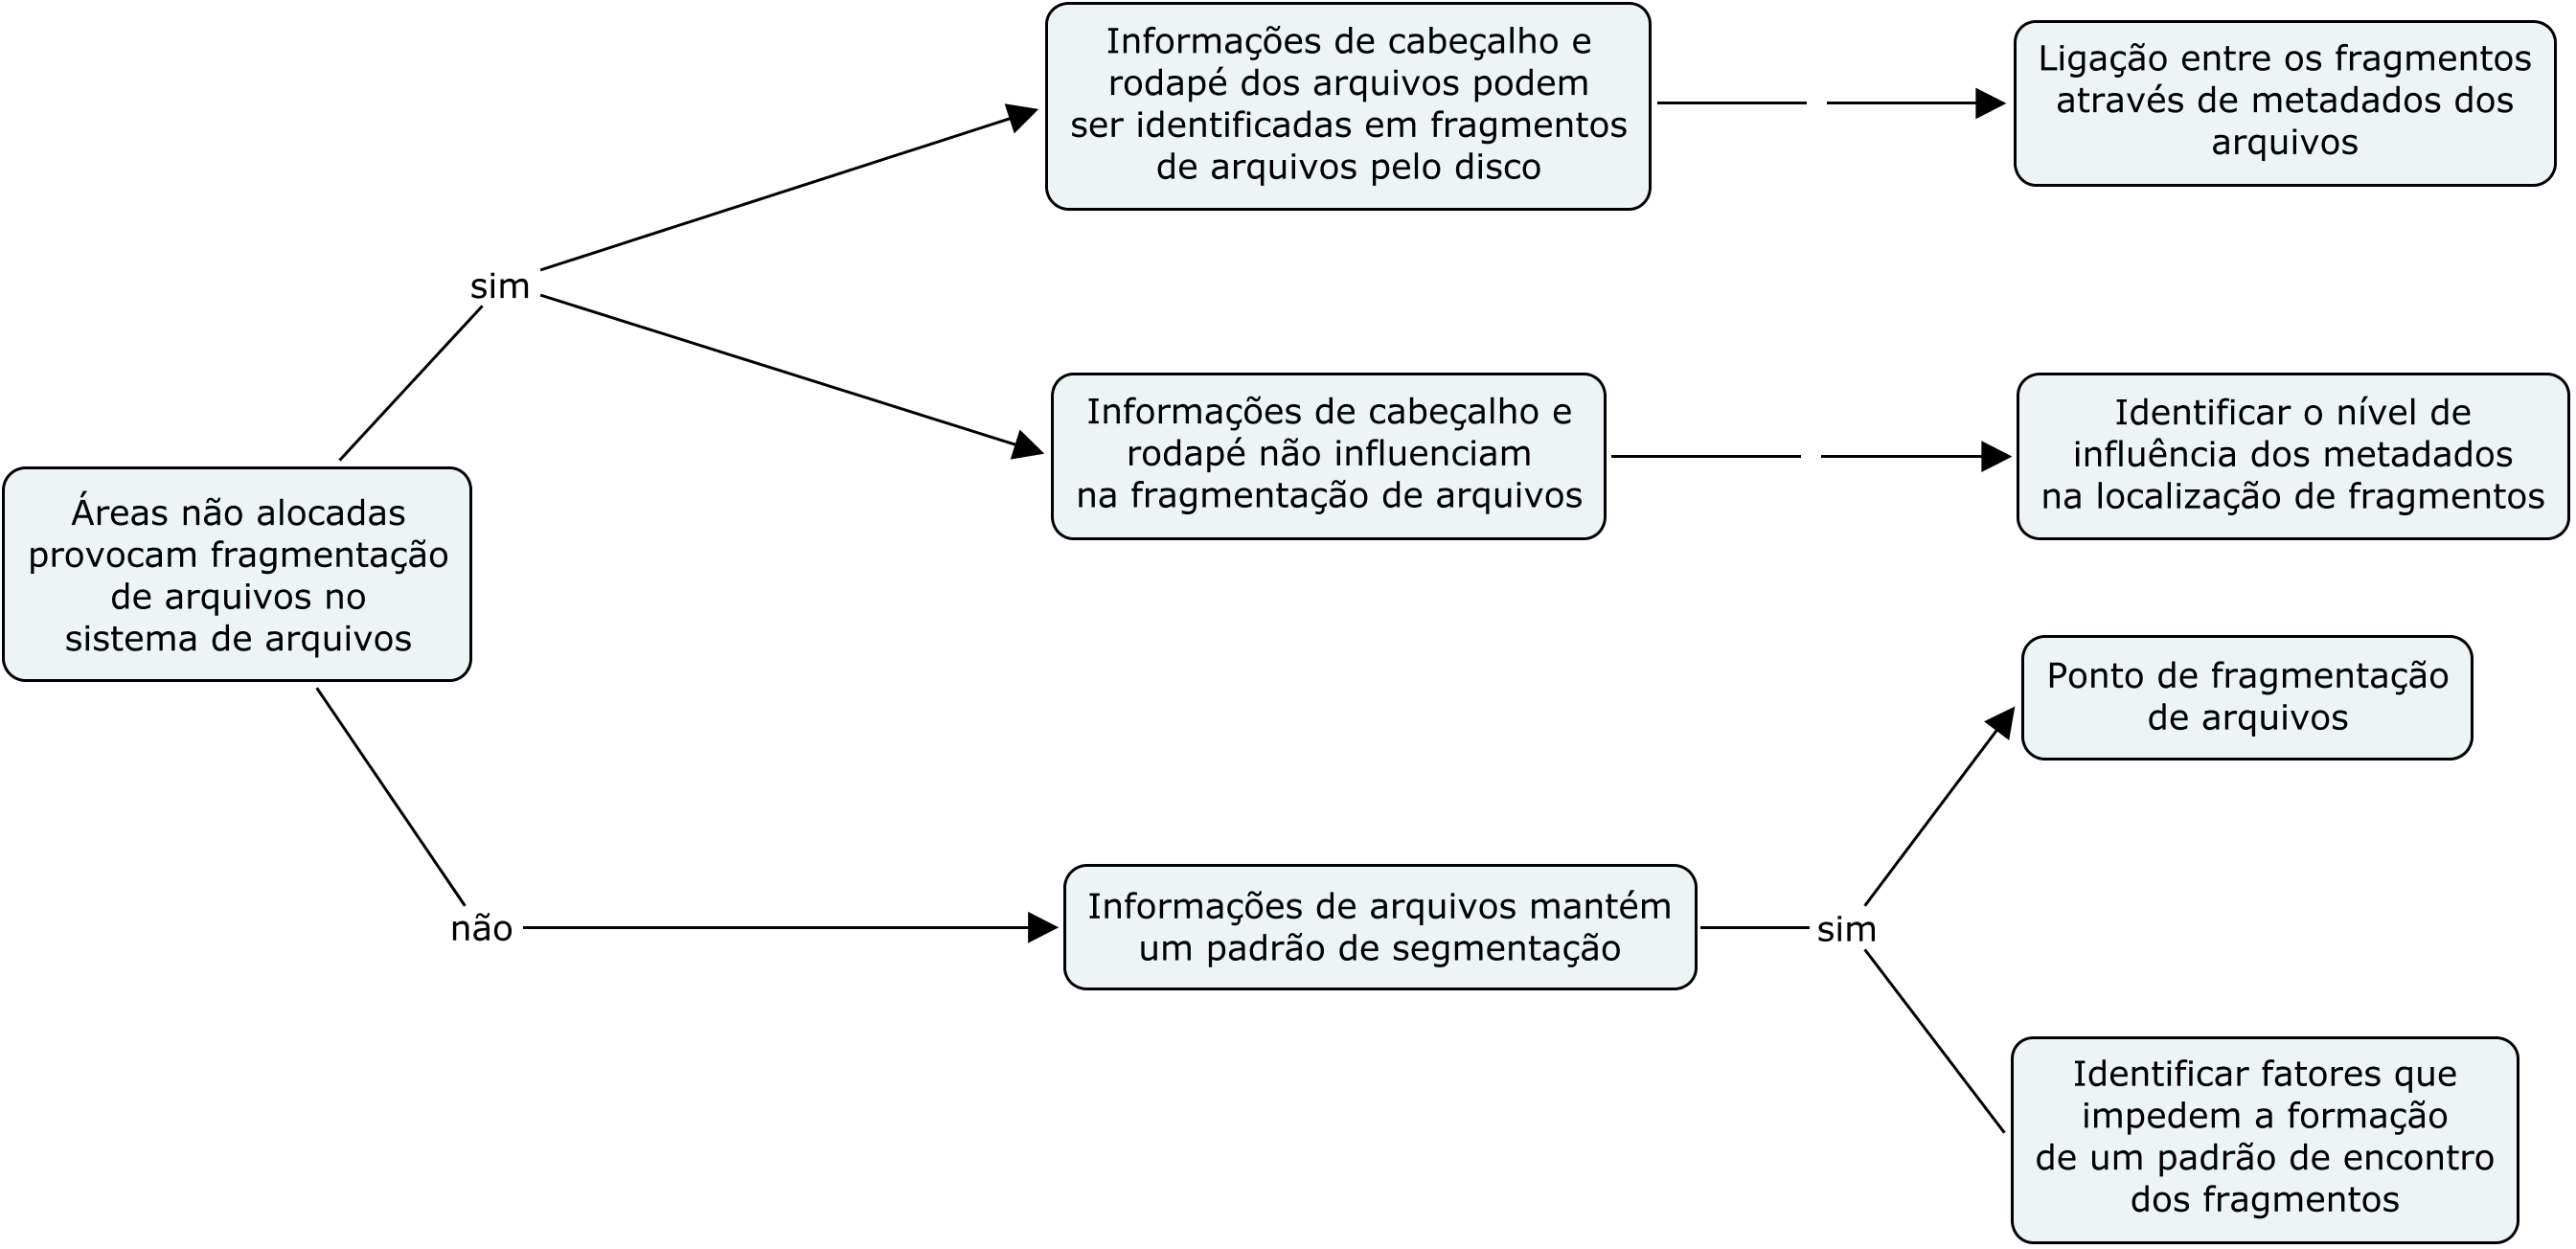
\includegraphics[scale=0.15]{figuras/hipotese.png}
  \caption{Hip�tese de pesquisa}
  \label{fig:hipotese}
\end{figure}

\section{Objetivo Geral}
Visto a necessidade de mitigar o impacto da fragmenta��o no processo de file carving em uma investiga��o digital, busca-se determinar uma melhor metodologia de localiza��o dos fragmentos de arquivos, esclarecer uma maneira de localiza��o dos fragmentos de um arquivo dentro da �rea n�o alocada em sistemas de arquivos NTFS.

\section{Objetivo Espec�fico}
Para chegar ao objetivo principal e determinar uma melhor metodologia de localiza��o de fragmentos de arquivos � necess�rio entender primeiramente e de forma mais detalhada alguns itens espec�ficos:

\begin{itemize}
 \item Verificar como s�o identificados os arquivos no sistema de arquivo NTFS.
 \item Verificar como um arquivo fragmentado � armazenado em um sistema NTFS.
 \item Levantar uma padroniza��o entre os fragmentos de arquivos para melhor localiza��o.
 \item Identificar formas de localiza��o de fragmentos dos arquivos n�o alocados.
 \item Verificar o uso de entropia para localiza��o de fragmentos de arquivos.
\end{itemize}

Verificar assim a forma como os arquivos s�o registrados nos sistemas de arquivos NTFS, o processo de diferencia��o de tipos de arquivos para determinar o in�cio e o fim de um arquivo (�rea de cabe�alho, �rea de dados, de metadados e ponto de fim de arquivo), podendo ent�o encontrar certos padr�es que possam permitir a identifica��o de partes de um arquivo fragmentado no sistema de arquivos.

\section{Metodologia}
Pesquisar e descrever o funcionamento do sistema de arquivos NTFS e identificar em sua estrutura de armazenamento de arquivos o ponto de fragmenta��o dos arquivos podendo dessa forma atingir o objetivo de determinar uma melhor forma de recupera��o dos fragmentos de arquivos em �reas n�o alocadas, atrav�s das bibliografias levantadas juntamente com pesquisas j� realizadas sobre assuntos correlatos � fragmenta��o de arquivos e file carving.

O m�todo de pesquisa utilizado � o embasamento nas defini��es de documenta��o do sistema de arquivos NTFS junto ao criador (Microsoft), pesquisas correlatas referentes � fragmenta��o de arquivos e sua forma de identifica��o, pesquisar a liga��o entre os fragmentos de dados para entender o ponto de fragmenta��o e identificar se h� um padr�o nessa rela��o de fragmentos de arquivos.

Para fins comprobat�rios, ser�o utilizados dois softwares amplamente utilizados com a finalidade de identifica��o de arquivos n�o alocados que ser�o testados sobre os mesmos par�metros para que se possa concretizar, atrav�s de dados significativos, a efic�cia do processo de identifica��o de fragmentos de arquivos n�o alocados. As ferramentas em quest�o utilizadas s�o o Foremost e Scalpel.
\chapter{Levantamento Bibliográfico}
Desenvolvimento do texto baseado nas referências pesquisadas, que corresponde ao corpo teórico do trabalho. Aqui, deve-se incluir a pesquisa bibliográfica dos assuntos relacionados ao tema, obtendo o corpo de conhecimentos que balizará o estudo. Os capítulos e subtítulos devem ser encadeados de forma a explicar, discutir e demonstrar o conteúdo do trabalho.
Esta etapa consiste em estruturar de maneira lógica as partes do trabalho, seus capítulos, de forma que estes estejam bem inseridos no contexto do discurso e da redação. Pode ser que, no decorrer do trabalho, esta construção lógica precise sofrer modificações ou desdobramentos, até que se chegue ao plano definitivo (Severino: 1979, p. 86). Toda a argumentação e raciocínio são construídos em cima das leituras, experiências e da vivência intelectual a respeito do problema da pesquisa.
Esta fase pressupõe o levantamento de toda a documentação existente sobre o assunto da pesquisa: livros, artigos, revistas. Conforme colocado por Severino (1979, p. 81), esta é a ”fase da heurística, ciência, técnica e arte da pesquisa de documentos”. 
É importante salientar que o trabalho, nesta etapa, pressupõe uma finalidade didática, não podendo ser uma pura criação mental do aluno. Deve se balizar em pesquisas e consultas de documentação, em livros, artigos técnicos e jornais, de forma a gerar quantidade suficiente de informação sobre o tema do trabalho. As idéias e opiniões dos alunos, da fase do levantamento bibliográfico, podem ajudar na ligação entre idéias de autores, mas não devem prevalecer sobre a pesquisa dos autores. 
É interessante que, antes de iniciar a leitura dos materiais, o aluno elabore um roteiro de trabalho (que podem ser a origem dos capítulos), ou seja, uma primeira estruturação, de forma que a leitura e a pesquisa se dêem dentro deste roteiro. Ou seja, tenha em mente quais são as colunas mestras do trabalho que demonstrarão, dos textos lidos, os elementos que devem ser retidos para o aproveitamento na composição do trabalho. Vale salientar que este roteiro é provisório, podendo ser reformulado no decorrer do trabalho.
O aluno deve proceder uma análise de possíveis materiais que podem ser interessantes para o estudo do tema e consultar seu orientador sobre livros que são imprescindíveis para a consecução do estudo. Algumas dicas válidas: tire um tempo para ir a biblioteca e analise os livros pelo seu índice. Muitas vezes, importantes teorias não aparecem no título da obra, mas sim em capítulos dos livros. Pesquisar com paciência, nesta fase, é a chave do sucesso futuro do trabalho. 
Procure analisar livros relacionados com o assunto, revistas, teses. Com certeza, esta atitude vai ajudar não apenas no estudo e detalhamento do tema em si, como também dar um foco mais interessante ao estudo ou ao problema de pesquisa. Lembre-se: pesquisar não significa perder tempo, mas sim, ganhar luz e maior proficiência sobre o assunto.
Uma última colocação acerca do levantamento bibliográfico: atualmente, os alunos tendem a pesquisar com ênfase errônea na Internet. Apesar de este ser um meio de informação altamente eficaz, certamente não é suficiente para gerar o conhecimento necessário ao desenvolvimento teórico do trabalho. Podemos comparar a Internet a um lago, que pode ser extenso, porém é raso, superficial.
Outro cuidado diz respeito à ação “copiar e colar”.  Nesta hora, o aluno deve ter amadurecimento necessário para não copiar trechos de obras, mesmo que contenha a citação da mesma, pois isso  se configura plágio. O trabalho deve ser o de ler e reformular o que foi dito pelo autor, dentro da perspectiva de seu tema. Um exemplo de reformulação: “Segundo Coda (ano), a motivação pode ser definida como...”. Perceba que, desta forma, o trecho do autor Coda não esta sendo copiado, mas comentado pelo autor da monografia.
Quando for absolutamente imprescindível copiar definições ou trechos de obras, este deve ser colocado entre aspas, de forma que fique clara a autoria de determinado trecho, e deve ser indicada a página do livro de onde foi retirada. Trechos com mais de 4 linhas devem vir em fonte menor e com margem esquerda de 4 cm.
A seguir, devem ser desenvolvidos os capítulos. Um ponto importante é fazer a ligação entre um capítulo e o seguinte, de forma que o leitor entenda completamente a sequenciação.

\chapter{Capítulo 1 - Sistemas de Arquivos}
...

\chapter{Capítulo 2 - NTFS}
...

\section{Conceito}
...

\section{Estrutura de Dados}
...

\section{Análise Típica}
...

\chapter{Capítulo 3 - File Carving}
...

\section{Conceito}
...

\section{Assinatura de Arquivo}
...

\section{Número Mágico}
...

\chapter{Capítulo 4 - File Carving Avançado}
...

\section{Conceito}
...

\section{Funcionamento}
...

\section{Fragmentação}
...

\section{Ponto de Fragmentação}
...aqui serão incluídos também algoritmos de detecção de pontos de fragmentação como listado no mind map (Sequential Hypothesis Testing)...



\chapter{Considera��es Finais}

Com base em todos os m�todos apresentados, inclusive a abordagem da an�lise de entropia na recupera��o e classifica��o de fragmentos de dados, a
conclus�o que se chega � que a recupera��o de dados fragmentados � e continua sendo um desafio para as investiga��es forenses, pela dificuldade de se
aplicar as t�cnicas, pela diferencia��o entre t�cnicas e tipos de aplica��o para tipos de arquivos diferenciados e pelo crescente volume de
informa��es presentes nas imagens investigadas. Tendo em vista sua complexidade e a variedade de situa��es em que os fragmentos podem se apresentar,
e a impossibilidade, at� o presente momento, da aplica��o de automa��o do processo em uma ferramenta objetiva de file carving, faz-se necess�ria a
abordagem de v�rias t�cnicas demonstradas nesta pesquisa e em diversas outras, o que demanda um tempo demasiado, incluindo an�lises manuais sobre
arquivos, sendo praticamente invi�vel em investiga��es forenses que usualmente n�o apresentam tempo suficiente para uma an�lise complexa dos dados
envolvidos.

Sendo assim, a escolha da abordagem ideal para localiza��o dos fragmentos depende de in�meros fatores que podem estar presentes na imagem investigada,
o tipo de sistema de arquivo, os tipos de arquivos mais comuns presentes na imagem investigada e os mais poss�veis de se apresentar provas concretas,
a situa��o do n�vel de fragmenta��o desses arquivos, as condi��es dessas informa��es presentes em slack space. Em grandes volumes de dados, analisar
esses quesitos baseado nas informa��es de dados presentes � uma tarefa muito complexa e custosa. Algumas ferramentas forenses tem voltado seus
olhos e estudos para a recupera��o de dados, tais como \emph{Foremost} e \emph{Scalpel}, que fazem uso de algumas destas t�cnicas para aproximar
cada vez mais as condi��es de recupera��o dos arquivos, conseguindo assim um resultado mais eficaz e satisfat�rio, o que n�o seria garantido
se utilizada uma ou outra abordagem.

A an�lise de entropia ainda est� sendo estudada com sua abordagem direcionada ao comportamento de diverg�ncia dos dados. Muito embora essa t�cnica
ainda apresente falhas nos processos de identifica��o de fragmentos, essa � uma das abordagens mais promissoras de melhoria de efic�cia no processo de
identifica��o e classifica��o de fragmentos de dados sendo necess�rio mais estudos para possibilitar a automatiza��o do processo para evitar a
necessidade de an�lises manuais sobre imagens forenses.
% \chapter{Cronograma}
...
% \chapter{Projeto de Sumário de TGI}
...
\chapter{Apêndice}
...
\chapter{Anexos}
...

\bibliography{bb}
\bibliographystyle{abnt-alf}

\end{document}
